% Created 2025-07-04 Fri 14:23
% Intended LaTeX compiler: pdflatex
\documentclass[11pt]{article}
\usepackage[utf8]{inputenc}
\usepackage[T1]{fontenc}
\usepackage{graphicx}
\usepackage{longtable}
\usepackage{wrapfig}
\usepackage{rotating}
\usepackage[normalem]{ulem}
\usepackage{amsmath}
\usepackage{amssymb}
\usepackage{capt-of}
\usepackage{hyperref}
\author{Leonardo Bizzoni}
\date{\today}
\title{Relazione Laboratori Coderbot\\\medskip
\large Gruppo: Leonardo Bizzoni (899629) - Camilla Cantaluppi (894557) - altri?}
\hypersetup{
 pdfauthor={Leonardo Bizzoni},
 pdftitle={Relazione Laboratori Coderbot},
 pdfkeywords={},
 pdfsubject={},
 pdfcreator={Emacs 30.1 (Org mode 9.7.11)}, 
 pdflang={English}}
\begin{document}

\maketitle
\tableofcontents

\section{Trasformazione delle letture encoder in lunghezze degli archi percorsi}
\label{sec:orgcf6fb9b}
L'ottenimento dei tick misurati da entrambi gli encoder, sinitro e destro, viene fatto tramite le 2 istanze di `cbEncoder\textsubscript{t}`:
\begin{verbatim}
cbEncoder_t cb_encoder_left = { PIN_ENCODER_LEFT_A, PIN_ENCODER_LEFT_B, -1 };
cbEncoder_t cb_encoder_right = { PIN_ENCODER_RIGHT_A, PIN_ENCODER_RIGHT_B, -1};
\end{verbatim}
e leggendo il valore del parametro `ticks`.

La conversione del valore in tick al suo corrispondente in millimetri percorsi viene fatto grazie a 2 variabili di conversione (\emph{una per encoder}) misurante in millimetri/tick.
Queste 2 variabili sono state trovate sperimentalmente cercando di far andare il coderbot in linea retta per un albitrario intervallo di tempo e misurando la distanza percorsa con un metro e osservando quanti tick erano stati misurati dai 2 encoder. Dopo aver ripetuto l'esperimento 6 volte questi sono i risultati ottenuti:
\begin{center}
\begin{tabular}{lrr}
distanza percorsa & tick encoder\textsubscript{sinistro} & tick encoder destro\\
\hline
91mm & 828 & 832\\
109mm & 965 & 970\\
98mm & 909 & 882\\
105mm & 891 & 941\\
98mm & 908 & 851\\
104mm & 925 & 938\\
\end{tabular}
\end{center}

\begin{itemize}
\item Media mm/tick encoder sinistro:            0.11147909938205335
\item Media mm/tick encoder destro:              0.1117455840579235
\item Varianza tick encoder sinistro:            1.4429498891258886e-5
\item Varianza tick encoder destro:              3.7696146281431147e-6
\item Deviazione standard tick encoder sinistro: 0.003798618023868534
\item Deviazione standard tick encoder destro:   0.0019415495430565542
\end{itemize}

Come costanti di conversione abbiamo utilizzato le 2 medie (\emph{MillimeterFromTicks\textsubscript{Left}, MillimeterFromTicks\textsubscript{Right}}) le quali sono misurate in millimetri su tick.
\section{Ciclo di controllo delle ruote}
\label{sec:org3f027c6}
Il controllo delle ruote inizia leggendo il valore di velocità delle singole ruote impostato dalla task di controllo cartesiano. Questa lettura viene effettuata in sezione critica per evitare corse critiche dove la task di controllo cartesiano sovrascrive il valore di velocità mentre la task di controllo ruote cerca di leggerlo:
\begin{verbatim}
os_mutex_lock(state.speed.mutex);
// (mm/s) / (mm/tick) = (mm/s) * (tick/mm) = tick/s
f32 target_ticksXsec_left = state.speed.left / MillimeterFromTicks_Left;
f32 target_ticksXsec_right = state.speed.right / MillimeterFromTicks_Right;
os_mutex_unlock(state.speed.mutex);

// (tick/s) * (ms / 1000ms) = tick
u64 target_ticks_left = target_ticksXsec_left * ((f32)period_ms / 1000.);
u64 target_ticks_right = target_ticksXsec_right * ((f32)period_ms / 1000.);
\end{verbatim}
Usando un approccio a 2 task, una per ogni ruota, si potrebbe sostituire il mutex lock con un rwlock per evitare di bloccare inutilmente le 2 task di sola lettura di controllo ruote.

La velocità è data in millimetri al secondo ed è quindi necessario convertirla in un valore di tick che aspettiamo verranno misurati dai 2 encoder.

`libcoderbot` non espone un lock per la lettura dei tick quindi lettura e scrittura possono avvenire in modo asincrono. Per evitare letture di tick sfasate, questi vengono salvati in altre 2 variabili protette da sezione critica per la condivisione con la task di odometria.
\begin{verbatim}
os_mutex_lock(state.tick.mutex);
state.tick.measured_left = cb_encoder_left.ticks;
state.tick.measured_right = cb_encoder_right.ticks;
os_mutex_unlock(state.tick.mutex);
\end{verbatim}

Dopodiche viene determinato il nuovo duty cycle dei motori in base all'errore tra tick misurati dagli encoder e tick attesi, scalato in base alle costante proporzionali `Kp\textsubscript{Left}`, `Kp\textsubscript{Right}` e con l'aggiunta dell'errore accumulato durante l'intera esecuzione della task, scalato in base alle costanti integrali `Ki\textsubscript{Left}`, `Ki\textsubscript{Right}`.
La nuova direzione è data dal segno del duty cycle:
\begin{itemize}
\item duty cycle negativo implica che il coderbot deve muoversi indietro
\item duty cycle positivo implica che il coderbot deve muoversi in avanti
\item duty cycle nullo implica che il coderbot restare fermo e quindi la direzione è irrilevante
\end{itemize}
\begin{verbatim}
i64 delta_left = target_ticks_left - state.tick.measured_left;
i64 delta_right = target_ticks_right - state.tick.measured_right;

accumalated_error_left += delta_left;
accumalated_error_right += delta_right;

duty_cycle_left = Kp_Left * delta_left + Ki_Left * accumalated_error_left;
duty_cycle_right = Kp_Right * delta_right + Ki_Right * accumalated_error_right;

motor_direction_left = duty_cycle_left < 0 ? backward : forward;
motor_direction_right = duty_cycle_right < 0 ? backward : forward;

duty_cycle_left = Clamp(Abs(duty_cycle_left), 0.1, 0.6);
duty_cycle_right = Clamp(Abs(duty_cycle_right), 0.1, 0.6);

cb_encoder_left.ticks = 0;
cb_encoder_right.ticks = 0;
cbMotorMove(&cb_motor_left, motor_direction_left, duty_cycle_left);
cbMotorMove(&cb_motor_right, motor_direction_right, duty_cycle_right);
\end{verbatim}

Trovare i valori delle costanti `Kp\textsubscript{Left}`, `Kp\textsubscript{Right}`, `Ki\textsubscript{Left}`, `Ki\textsubscript{Right}` è anchesso stato fatto in maniera sperimentale separatamente.
Per le costanti proporzionali si è cercato di trovarle andado a modificarle leggermente ad ogni esecuzione del programma cercando di aggiustarle per far andare il coderbot dritto. Una volta trovate queste, si è passati alle costanti integrali che, analogamente, sono state regolate gradualmente con l'obiettivo di ridurre il delta tra i tick desiderati e tick misurati.
\section{Odometria}
\label{sec:orgf92f562}
\subsection{Rappresentazione delle pose del robot}
\label{sec:org5b5d30e}
\begin{center}
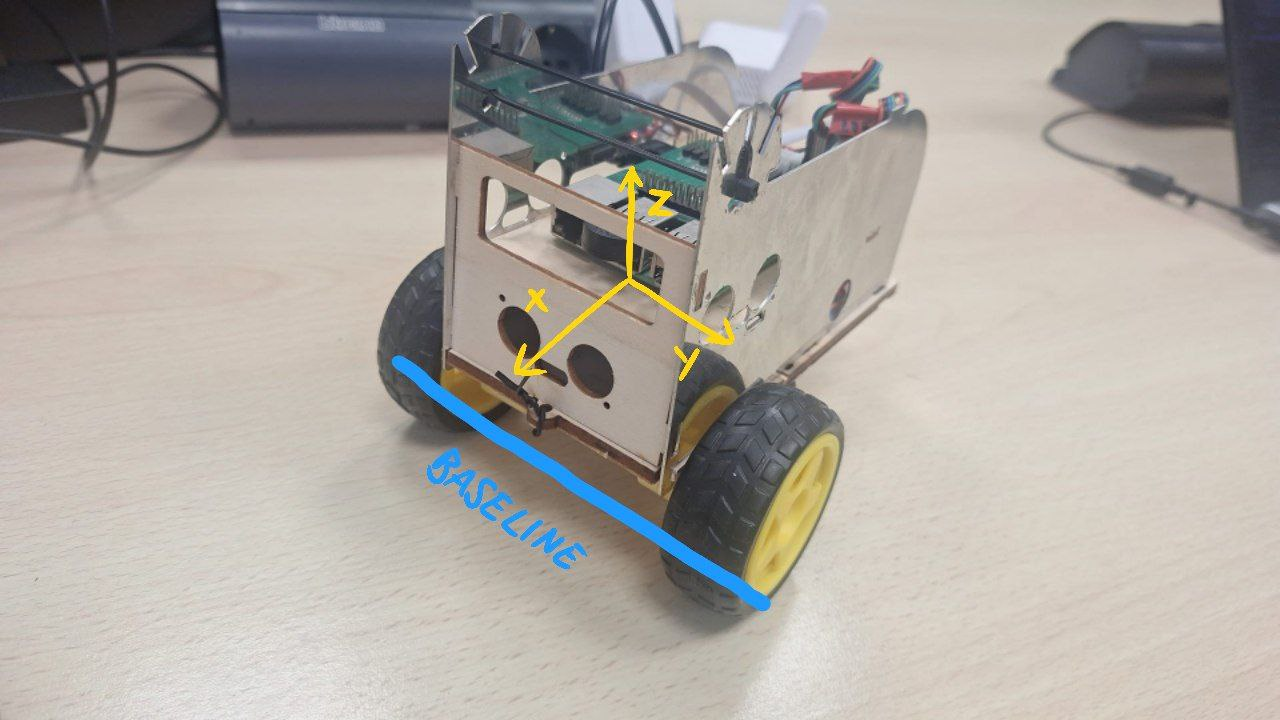
\includegraphics[width=300]{/home/leo/Pictures/coderbot-graph.jpg}
\end{center}

La pose del coderbot (\emph{la sua rotazione e posizione corrente}) viene modellata tramite una matrice \(3\times3\)  \(\text{pose}=\begin{bmatrix}R_{xx}&R_{yx}&P_x\\R_{xy}&R_{yy}&P_y\\0&0&1\end{bmatrix}\), dove:
\begin{itemize}
\item \(\bold R_{x}\) è il versore dell'asse X del sistema di riferimento attaccato al corpo del coderbot.
\item \(\bold R_{y}\) è il versore dell'asse Y del sistema di riferimento attaccato al corpo del coderbot.
\item \(\bold P\) è il vettore che indica la posizione del coderbot rispetto all'origine del sistema di riferimento attaccato al corpo del coderbot.
\end{itemize}
\subsection{Comporamente della task periodica}
\label{sec:orgd742f41}
Nella task di odometria vengono letti i tick misurati dagli encoder e, grazie alle costanti di conversione da tick a millimetri, si ottiene la distanza percorsa dal coderbot nel tempo percorso tra l'attivazione precedente e quella corrente della task di odometria:
\begin{verbatim}
f32 distance_left = ticks_left * MillimeterFromTicks_Left;
f32 distance_right = ticks_right * MillimeterFromTicks_Right;
\end{verbatim}

Sapendo la distanza percorsa dalle 2 ruote e la distanza tra di esse è possibile determinare l'angolo di rotazione rispetto al centro di istantanea rotazione:
\begin{verbatim}
f32 delta_theta = -(distance_left - distance_right) / BASELINE_MM;
\end{verbatim}
Per rispettare la convenzione secondo cui le rotazioni in senso antiorario hanno segno positivo, viene invertito il segno dell'angolo.

\begin{center}
\rule[1ex]{.5\textwidth}{.5pt}
\end{center}

Se l'angolo \(\theta\) è minore di una certa soglia, da noi fissata a \(0.005\text{rad}\), allora dato che la rotazione misurata è prossochè nulla, possiamo approssimare il movimento ad una linea retta lungo l'asse delle \(X\) con modulo uguale alla media delle distanze percorse dalle 2 ruote.
L'operazione da applicare alla pose attuale del coderbot sarà una semplice traslazione lungo l'asse delle X, \(\text{pose}=\text{pose}\cdot\begin{bmatrix}R&P\\0^T&1\end{bmatrix}\) dove:
\begin{itemize}
\item \(R=I_2=\begin{bmatrix}1&0\\0&1\end{bmatrix}\)
\item \(P= \begin{bmatrix}(\text{distance left} - \text{distance right})/2\\0\end{bmatrix}\)
\end{itemize}

Viceversa, se l'angolo \(\theta\) è maggiore della soglia, questo indica che il coderbot sta effettivamente curvando rispetto a un centro di istantanea rotazione (\emph{anche detto CIR}).
\end{document}
